\chapter{Fallstudie Project Planning}

In einer konkreten Fallstudie ging es um eine Planung eines Projekts, welche wie folgt gegliedert ist:
\begin{itemize}
	\item Geschäftsanalyse (Firma und Umfeld verstehen)
	\item Arbeitspakete (APs definieren und schätzen)
	\item Teamplanung (Teamzusammenstellung aufgrund von Profilen, Zuordnung von APs)
	\item Ressourcenplanung (Mitarbeiterplanung)
	\item Meilensteinplanung
\end{itemize}

\section{Geschäftsanalyse}
Bei der Analyse des Geschäfts müssen wir einmal mehr die Projektziele sowie die Anforderungen verstehen. Eine Anforderung ist eine Soll-Aussage über ein System oder einen Prozesse, welche eine Leistung oder eine Eigenschaft beschreibt. Anforderungen klar, einfach und messbar definieren. ''Antwortzeit des Dialogs in 97\% der Fälle unter 3 sec.''. Zielformulierungen und Anforderungen müssen demnach vorhanden sein.

\section{Arbeitspakete}
Mittels Anforderungen, Projektergebnisse und den Teilresultaten werden wir APs erstellen und die Aufwände für die APs schätzen.

\begin{itemize}
	\item Mapping aller Anforderungen zu den Resultaten. Damit keine Anforderungen vergessen gehen. Nebenbei können daraus die meisten APs definiert werden.
	\item Ein AP sollte in einer halben bis zwei Wochen abzuarbeiten sein und maximal 20 PT betragen. Somit brechen wir die Ergebnisse herunter. 
\end{itemize}

\subsection{Aufwandschätzung}
\label{sec:aufwandschaetzung}
In der Informatik unterschätzt man den Aufwand gerne! Also Achtung mit grosszügigen Schätzungen. Da sich ein Projekt im Laufe der Zeit ändert, muss man es auch kontrollieren. An folgenden Faktoren lässt sich schrauben, aber nicht unabhängig voneinander!

\begin{figure}[h!]
\centering
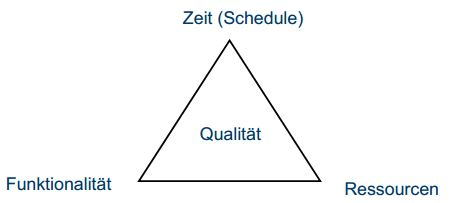
\includegraphics[width=0.3\linewidth]{fig/schaetzung-dreieck}
\caption{Schätzungs-Dreieck}
\label{fig:schaetzung-dreieck}
\end{figure}

Nachfolgend einige Schätzmethoden:
\begin{itemize}
	\item Individual Expert Judgmetn (WBS - Work Break Down Structure)
	\item Estimation by Analogy
	\item Count, Compute, Judge (Function Point Methode)
	\item Expert Judgment in Groups
	\item Formale Methoden
\end{itemize}

\paragraph{WBS} Projekt wird in APs unterteilt. Diese APs werden geschätzt. Diese ist am weitesten verbreitete Schätzmethode, oft sind es keine Schätzexperten und oft hat man keine Grundlage zum Schätzen. Kann erfolgreich sein, sollte aber nach Möglichkeit durch andere Methode ergänzt werden.

Best Practices: Projekt-durchführende Personen sollen schätzen. Tasks möglichst weit herunter brechen. Bei Unsicherheit bester und schlechtester Wert schätzen und Mittelwert nehmen. Alternativ kann auch eine Reserve von 10\% - 20\% hinzugezogen werden. Während dem Projekt aktuelle Resultate aufnehmen und vergleichen.

Wenn man die Implementation (inkl. Testing) schätzen muss, dann kann man im Normalfall den Wert fürs Design mal 2 rechnen.

Timeboxing bedeutet, dass der Zeitrahmen fix ist und der Scope vom Projekt angepasst werden darf.

\section{Ressourcenplanung}
\label{sec:ressourcenplanung}
Unter Ressourcenplanung verstehen wir die Zuordnung der Arbeitspakete zu den Projekt-Mitarbeiter und die Verteilung der Aufwände über die Zeit. Nachfolgende Aufzählung zeigt das Vorgehen bei der Ressourcenplanung:
\begin{enumerate}
	\item Festlegung der für die Arbeiten benötigten Profile und Zuordnung zu den Arbeitspaketen.
	\item Prüfen, welche Arbeitspakete parallel bearbeitet werden können. AP in Gruppen zusammenfassen. Alle AP einer Gruppe können parallel bearbeitet werden.
	\item 
	\begin{enumerate}
		\item Sichtung der verfügbaren Mitarbeiter und deren Profile und Zuordnung Mitarbeiter $\leftrightarrow$ Arbeitspaketen und ...
		\item Verteilung der Aufwände pro Arbeitspakete und Mitarbeiter auf die verfügbare Zeit und Beachtung der Auslastung der Mitarbeiter.
	\end{enumerate}
\end{enumerate}

\section{Meilensteinplanung}
\label{sec:meilensteinplanung}
Meilensteine sind wichtige Eckpunkte. Pro Meilenstein definiert man, welche Resultate erledigt sein müssen. Dies dient auch als Controlling-Punkt. Man kann genau sagen, wie weit der Projektfortschritt ist. Falls man nicht im Plan ist, kann man geeignete Massnahmen einleiten.

\section{Was ist der kritische Pfad in einem Projekt?}
Längster zeitlicher Pfad wo die Arbeitspakete hintereinander (seriell) gemacht werden müssen. Bestimmt wie lange das Projekt mindestens dauert.


\section{Lernziele}

\subsection{Sie sind in der Lage, aus der Beschreibung der Ausgangslage und dem Anforderungskatalog eines Projektes Teilresultate und Arbeitspakete für ein Projekt zu definieren.}
Siehe Abschnitt \ref{sec:aufwandschaetzung}

\subsection{Sie können auf Grundlage einer Arbeitspaketliste eine Teamplanung für ein Projekt durchführen.}
Siehe Abschnitt \ref{sec:ressourcenplanung}

\subsection{Auf der Basis der Arbeitspakete und der Teamplanung sind sie im Stande, eine Meilensteinplanung zu erstellen.}
Siehe Abschnitt \ref{sec:meilensteinplanung}
